\documentclass[11pt, article, one side]{memoir}

\settrims{0pt}{0pt} % page and stock same size
\settypeblocksize{*}{34.5pc}{*} % {height}{width}{ratio}
\setlrmargins{*}{*}{1} % {spine}{edge}{ratio}
\setulmarginsandblock{1in}{1in}{*} % height of typeblock computed
\setheadfoot{\onelineskip}{2\onelineskip} % {headheight}{footskip}
\setheaderspaces{*}{1.5\onelineskip}{*} % {headdrop}{headsep}{ratio}
\checkandfixthelayout


%-------- Packages --------%

\usepackage{mathtools}
\usepackage{amsthm}
%\usepackage{amssymb}
\usepackage{dutchcal}
\usepackage{newpxtext}
\usepackage[varg,bigdelims]{newpxmath}
%\usepackage{eucal}
%\usepackage[usenames,dvipsnames]{xcolor}
\usepackage{tikz}
%\usepackage[siunitx]{circuitikz}
%\usepackage{graphicx}
%\usepackage{outline}
%\usepackage{varwidth}
\usepackage[inline]{enumitem}
%\usepackage{ifthen}
%\usepackage[utf8]{inputenc} %allows non-ascii in bib file
\usepackage[bookmarks=true, colorlinks=true, linkcolor=blue!50!black,
citecolor=orange!50!black, urlcolor=orange!50!black, pdfencoding=unicode]{hyperref}
\usepackage[capitalize]{cleveref}
\usepackage[backend=biber, backref=true, maxbibnames = 10, style = alphabetic]{biblatex}
%\usepackage[framemethod=tikz]{mdframed}
%\usepackage{todonotes}

%-------- Package setup --------%

% cleveref %
  \newcommand{\creflastconjunction}{, and\nobreakspace} % serial comma

% biblatex %
  \addbibresource{Library20180913.bib} 

% makeidx %
  \makeindex 

% hyperref %
  \hypersetup{final}

% enumitem %
  \setlist{nosep}
  

% tikz %
  \usetikzlibrary{ 
  	cd,
  	math,
  	decorations.markings,
		decorations.pathreplacing,
  	positioning,
  	arrows.meta,
  	shapes,
		shadows,
		shadings,
  	calc,
  	fit,
  	quotes,
  	intersections,
    circuits,
    circuits.ee.IEC
  }
  
	\tikzcdset{arrow style=tikz, diagrams={>=To}}

% mdframed/tablefootnote%
% This makes \tablefootnote allow construction of footnotes that appear at bottom of page instead of inside frame


%\mdfdefinestyle{exerciseframe}{
%    linecolor=white!93!yellow,
%    backgroundcolor=white!93!yellow,
%    }


% amsthm %
  \theoremstyle{theorem}
  \newtheorem{theorem}[equation]{Theorem}
  \newtheorem{proposition}[equation]{Proposition}
  \newtheorem{corollary}[equation]{Corollary}
  \newtheorem{lemma}[equation]{Lemma}
  
  \theoremstyle{definition}
  \newtheorem{definition}[equation]{Definition}
  \newtheorem{notation}[equation]{Notation}
  \newtheorem{axiom}{Axiom}
  \newtheorem*{axiom*}{Axiom}
  
  \theoremstyle{remark}
  \newtheorem{example}[equation]{Example}
  \newtheorem{remark}[equation]{Remark}
  \newtheorem{warning}[equation]{Warning}
%  \newtheorem{exercise}[equation]{Exercise}

% Adjunctions
\newcommand{\adj}[5][30pt]{%[size] Cat L, Left, Right, Cat R.
\begin{tikzcd}[ampersand replacement=\&, column sep=#1]
  #2\ar[r, bend left=15, shift left=2pt, "#3"]
  \ar[r, Rightarrow, shorten <=8pt, shorten >=8pt]\&
  #5\ar[l, bend left=15, shift left=2pt, "#4"]
\end{tikzcd}
}

\newcommand{\adjr}[5][30pt]{%[size] Cat R, Right, Left, Cat L.
\begin{tikzcd}[ampersand replacement=\&, column sep=#1]
  #2\ar[r, bend left=15, shift left=2pt, "#3"]\&
  #5\ar[l, bend left=15, shift left=2pt, "#4"]
  \ar[l, Rightarrow, shorten <=8pt, shorten >=8pt]
\end{tikzcd}
}

  
%-------- Single symbols --------%
	
\DeclareSymbolFont{stmry}{U}{stmry}{m}{n}
\DeclareMathSymbol\fatsemi\mathop{stmry}{"23}

\DeclareFontFamily{U}{mathx}{\hyphenchar\font45}
\DeclareFontShape{U}{mathx}{m}{n}{
      <5> <6> <7> <8> <9> <10>
      <10.95> <12> <14.4> <17.28> <20.74> <24.88>
      mathx10
      }{}
\DeclareSymbolFont{mathx}{U}{mathx}{m}{n}
\DeclareFontSubstitution{U}{mathx}{m}{n}
\DeclareMathAccent{\widecheck}{0}{mathx}{"71}


%-------- Renewed commands --------%

\renewcommand{\ss}{\subseteq}

%-------- Other Macros --------%

\DeclarePairedDelimiter{\pair}{\langle}{\rangle}
\DeclarePairedDelimiter{\copair}{[}{]}
\DeclarePairedDelimiter{\floor}{\lfloor}{\rfloor}
\DeclarePairedDelimiter{\ceil}{\lceil}{\rceil}

\DeclarePairedDelimiter{\corners}{\ulcorner}{\urcorner}




\DeclareMathOperator{\Hom}{Hom}
\DeclareMathOperator{\Mor}{Mor}
\DeclareMathOperator{\dom}{dom}
\DeclareMathOperator{\cod}{cod}
\DeclareMathOperator*{\colim}{colim}
\DeclareMathOperator{\im}{im}
\DeclareMathOperator{\ob}{Ob}
\DeclareMathOperator{\Tr}{Tr}
\DeclareMathOperator{\dju}{\sqcup}
\DeclareMathOperator{\plpl}{+\!+}

\DeclareMathOperator{\const}{\mathtt{const}}

\newcommand{\Set}[1]{\mathrm{#1}}%a named set
\newcommand{\cat}[1]{\mathcal{#1}}%a generic category
\newcommand{\Cat}[1]{\mathsf{#1}}%a named category
\newcommand{\fun}[1]{\textit{#1}}%function
\newcommand{\Fun}[1]{\mathbf{#1}}%functor
\newcommand{\type}[1]{\texttt{#1}}

\newcommand{\id}{\mathrm{id}}
\newcommand{\cocolon}{:\!}
\newcommand{\iso}{\cong}
\newcommand{\too}{\longrightarrow}
\newcommand{\tto}{\rightrightarrows}
\newcommand{\To}[1]{\xrightarrow{#1}}
\newcommand{\Tto}[3][13pt]{\begin{tikzcd}[sep=#1, cramped, ampersand replacement=\&, text height=1ex, text depth=.3ex]\ar[r, shift left=2pt, "#2"]\ar[r, shift right=2pt, "#3"']\&{}\end{tikzcd}}
\newcommand{\Too}[1]{\xrightarrow{\;\;#1\;\;}}
\newcommand{\from}{\leftarrow}
\newcommand{\From}[1]{\xleftarrow{#1}}
\newcommand{\Fromm}[1]{\xleftarrow{\;\;#1\;\;}}
\newcommand{\surj}{\twoheadrightarrow}
\newcommand{\inj}{\rightarrowtail}
\newcommand{\wavyto}{\rightsquigarrow}
\newcommand{\lollipop}{\multimap}
\newcommand{\pr}{\mathrm{pr}}
\newcommand{\tickar}{\begin{tikzcd}[baseline=-0.5ex,cramped,sep=small,ampersand 
replacement=\&]{}\ar[r,tick]\&{}\end{tikzcd}}
\newcommand{\imp}{\Rightarrow}
\renewcommand{\iff}{\Leftrightarrow}
\renewcommand{\th}{\ensuremath{^\tn{th}}\ }
\newcommand{\down}{\mathbin{\downarrow}}
\newcommand{\then}{\mathbin{\scalebox{.8}{/\!\!/}}}
\newcommand{\op}{^\tn{op}}
\newcommand{\grph}[1]{{#1}_{\mathrm{Gr}}}

\newcommand{\tn}[1]{\textnormal{#1}}
\newcommand{\ol}[1]{\overline{#1}}
\newcommand{\ord}[1]{\underline{#1}}
\newcommand{\wt}[1]{\widetilde{#1}}
\newcommand{\wh}[1]{\widehat{#1}}
\newcommand{\ubar}[1]{\underaccent{\bar}{#1}}
\newcommand{\LMO}[2][over]{\ifthenelse{\equal{#1}{over}}{\overset{#2}{\bullet}}{\underset{#2}{\bullet}}}
\newcommand{\LTO}[2][\bullet]{\overset{\tn{#2}}{#1}}


\newcommand{\bb}{\mathbb{B}}
\newcommand{\nn}{\mathbb{N}}
%\newcommand{\PP}{\mathbb{P}}
\newcommand{\zz}{\mathbb{Z}}
\newcommand{\rr}{\mathbb{R}}
\newcommand{\oo}{\mathcal{O}}
\newcommand{\singleton}{\{1\}}
\newcommand{\powset}{\Fun{P}}
\newcommand{\upset}{\Fun{U}}

\newcommand{\foo}{\const{foo}}
\newcommand{\true}{\const{true}}
\newcommand{\false}{\const{false}}

\newcommand{\inv}{^{-1}}

\newcommand{\boxCD}[2][black]{\fcolorbox{#1}{white}{\begin{varwidth}{\textwidth}\centering #2\end{varwidth}}}

\newcommand{\lo}[2]{#1(\,\cdot\,)^{#2}}

\newcommand{\smset}{\Cat{Set}}
\newcommand{\smcat}{\Cat{Cat}}
\newcommand{\finset}{\Cat{FinSet}}
\newcommand{\lens}{\Cat{Lens}}
\newcommand{\core}{\Fun{Core}}
\newcommand{\bun}{\Cat{Bun}}
\newcommand{\shv}{\Cat{Shv}}


\newcommand{\yon}{\mathcal{y}}
\newcommand{\poly}{\Cat{Poly}}
\newcommand{\dir}{\Cat{Dir}}

\newcommand{\qand}{\quad\text{and}\quad}
\newcommand{\qqand}{\qquad\text{and}\qquad}



\newcommand{\cp}{\mathbin{\fatsemi}}

%%fakesubsubsection generators
%}

\linespread{1.15}
%\allowdisplaybreaks
\setsecnumdepth{subsubsection}
\settocdepth{subsection}
\setlength{\parindent}{15pt}
\setcounter{tocdepth}{2}
\setlength{\parskip}{0em}

\begin{document}

\title{Polynomials, sheaves, and sums of co-representables\\Dirichlets, bundles, and sums of representables}

\author{David(s?)}

\maketitle

Polynomials $P(\yon)$ and finite Dirchlet series $D(\yon)$ in one variable $\cat{y}$, with natural number coefficients $a_i\in\nn$, are resectively functions of the form
\[
  P(\yon)=a_n\yon^n+\cdots+a_2\yon^2+a_1\yon^1+a_0\yon^0
  \qqand
  D(\yon)=a_nn^\yon+\cdots+a_22^\yon+a_11^\yon+a_00^\yon.
\]
There are of course infinite versions of the above, but in this paper we work entirely in the topos $\finset$ of finite sets, to keep things simple.

Recall that a \emph{co-representable functor} $\finset\to\finset$ is one of the form $\finset(s, -)$ for some finite set $s$; we denote this functor by $\yon^s$ and say it is co-represented by $s\in\finset$. Similarly, a \emph{co-representable functor} $\finset\op\to\finset$ is one of the form $\finset(-,s)$; we denote this functor by $s^\yon$ and say it is represented by $s$.
\[
  \yon^s \coloneqq \finset(s,-)
  \qqand
  s^\yon\coloneqq\finset(-,s).
\]
Note that the functor $0^\yon$ is not the constant $0$ functor; it is given by
\[
0^\yon(s)=
\begin{cases}
1&\tn{ if } s=0\\
0&\tn{ if } s\geq1.
\end{cases}
\]

A \emph{polynomial functor} \cite{GambinoKock} is a functor $P\colon\finset\to\finset$ that can be expressed as a finite sum of co-representable functors. Similarly, we define a \emph{Dirichlet functor} to be a functor $D\colon\finset\op\to\finset$ that can be expressed as a finite sum of representable functors:
\[
  P=\sum_{i\in P(1)}\yon^{p_i}
  \qqand
  D=\sum_{i\in D(0)}(d_i)^\yon.
\]

For any small category $C$, let $\finset^C$ denote the category whose objects are the functors $C\to\finset$ and whose morphisms are the natural transformations between them.

\begin{definition}
The \emph{category of polynomial functors}, denoted $\poly$, is the full subcategory of $\finset^\finset$ spanned by finite sums $P$ of corepresentables. The \emph{category of Dirichlet functors}, denoted $\dir$, is the full subcategory of $\finset^{(\finset\op)}$ spanned by the finite sums $D$ of representables.
\end{definition}

\begin{remark}

\end{remark}

There is a bijection between the respective object-sets of these two categories
\begin{align}
\nonumber
	\ob(\poly)&\To{\cong}\ob(\dir)\\\label{eqn.poly_dir}
	\sum_{i=1}^n\yon^{k_i}&\mapsto\sum_{i=1}^n (k_i)^\yon
\end{align}
In fact, these are further in bijection with the set of maps between finite sets.
\begin{proposition}\label{prop.poly_function}
There is a one-to-one correspondence between the set of polynomials in one variable, the set of finite Dirichlet series, and the set of (isomorphism classes of) functions $\pi\colon s\to t$ between finite sets.
\end{proposition}
\begin{proof}
We already established a bijection between polynomials and finite Dirichlet series in \cref{eqn.poly_dir}.

Given a polynomial $P=a_n\yon^n+\cdots+a_0$, we first define a pair of sets and a function $\pi\colon s\to t$ between them. Let $t\coloneqq P(1)=a_n+\cdots+a_0$, let $s\coloneqq\sum_{i=1}^na_i*i$. An element in $s$ can be written in the form $(i,j)$ where $1\leq i\leq n$ and $1\leq j\leq a_i*i$. Thus we may define $\pi(i,j)\coloneqq i$.

Given a function $\pi\colon s\to t$, we obtain a polynomial $P\coloneqq\sum_{i=1}^{t}\pi\inv(i)$. It is easy to see that the roundtrip for polynomials is identity, and that the round-trip for functions is a natural isomorphism.
\end{proof}

\begin{example}
The polynomial $2\yon^5+\yon^4+\yon^2+3$ corresponds to the function
\begin{equation}\label{eqn.bundle}
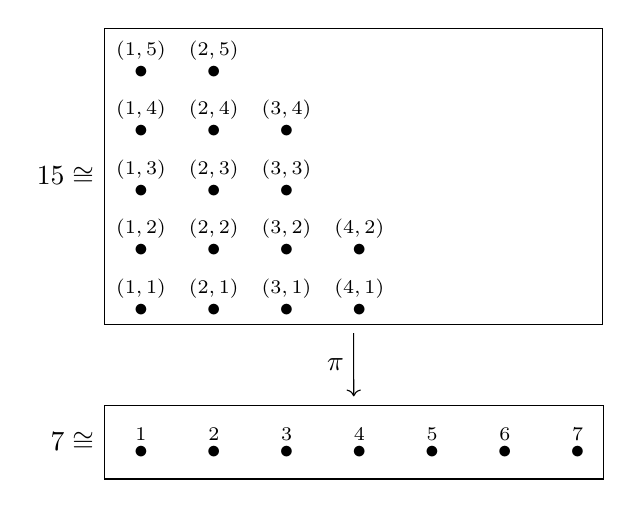
\begin{tikzpicture}[x=.5cm, y=.35cm, every label/.style={font=\scriptsize}, baseline=(f)]
	\node[label={[above=-5pt]:$1$}] (Ya) {$\bullet$};
	\node[right=1 of Ya,  label={[above=-5pt]:$2$}] (Yb) {$\bullet$};
	\node[right=1 of Yb,  label={[above=-5pt]:$3$}] (Yc) {$\bullet$};
	\node[right=1 of Yc,  label={[above=-5pt]:$4$}] (Yd) {$\bullet$};
	\node[right=1 of Yd,  label={[above=-5pt]:$5$}] (Ye) {$\bullet$};
	\node[right=1 of Ye,  label={[above=-5pt]:$6$}] (Yf) {$\bullet$};
	\node[right=1 of Yf,  label={[above=-5pt]:$7$}] (Yg) {$\bullet$};
	\node[draw, inner ysep=4pt, fit={($(Ya)+(-1em,3ex)$) (Yg)}] (Y) {};
	\node[left=0 of Y] (Ylab) {$7\cong$};
%
  \node[above=4 of Ya, label={[above=-5pt]:$(1,1)$}] (X11) {$\bullet$};
  \node[above=1 of X11, label={[above=-5pt]:$(1,2)$}] (X12) {$\bullet$};
  \node[above=1 of X12, label={[above=-5pt]:$(1,3)$}] (X13) {$\bullet$};
  \node[above=1 of X13, label={[above=-5pt]:$(1,4)$}] (X14) {$\bullet$};
  \node[above=1 of X14, label={[above=-5pt]:$(1,5)$}] (X15) {$\bullet$};
%
  \node[above=4 of Yb, label={[above=-5pt]:$(2,1)$}] (X21) {$\bullet$};
  \node[above=1 of X21, label={[above=-5pt]:$(2,2)$}] (X22) {$\bullet$};
  \node[above=1 of X22, label={[above=-5pt]:$(2,3)$}] (X23) {$\bullet$};
  \node[above=1 of X23, label={[above=-5pt]:$(2,4)$}] (X24) {$\bullet$};
  \node[above=1 of X24, label={[above=-5pt]:$(2,5)$}] (X25) {$\bullet$};
%
  \node[above=4 of Yc, label={[above=-5pt]:$(3,1)$}] (X31) {$\bullet$};
  \node[above=1 of X31, label={[above=-5pt]:$(3,2)$}] (X32) {$\bullet$};
  \node[above=1 of X32, label={[above=-5pt]:$(3,3)$}] (X33) {$\bullet$};
  \node[above=1 of X33, label={[above=-5pt]:$(3,4)$}] (X34) {$\bullet$};
%
  \node[above=4 of Yd, label={[above=-5pt]:$(4,1)$}] (X41) {$\bullet$};
  \node[above=1 of X41, label={[above=-5pt]:$(4,2)$}] (X42) {$\bullet$};
  \node [above=4 of Yg] (xend) {};
	\node[draw, inner ysep=3pt, fit={($(X15)+(-1em,3ex)$) ($(xend)+(.4,0)$)}] (X) {};
	\node[left=0 of X] {$15\cong$};
%
	\draw[->, shorten <=3pt, shorten >=3pt] (X) to node[left] (f) {$\pi$} (Y);
\end{tikzpicture}
\end{equation}
\end{example}

We can think of a function $\pi\colon s\to t$, e.g.\ that shown in \eqref{eqn.bundle}, as a bundle. We can also think of it as a sheaf. Sheaves and bundles are often considered to be synonymous, and indeed on objects they are. But in \cref{def.sheaves_bundles} we define bundle morphisms and sheaf morphisms to have different variances. 

For any function $f\colon t\to t'$ and function $\pi'\colon s'\to t'$, denote by $f^*(\pi')$ the pullback function as shown
\[
\begin{tikzcd}
	s\times_{t'}s'\ar[r]\ar[d, "f^*(\pi')"']&
	s'\ar[d, "\pi"]\\
	t\ar[r, "f"']&
	t'\ar[ul, phantom, very near end, "\lrcorner"]
\end{tikzcd}
\]

\begin{definition}\label{def.sheaves_bundles}
Let $\pi\colon s\to t$ and $\pi'\colon s'\to t'$ be functions between finite sets.
\begin{itemize}
	\item a \emph{bundle morphism} consists of a pair $(f,f_\sharp)$ where $f\colon t\to t'$ and $f_\sharp\colon s\to f^*(\pi')$ are functions;
	\item a \emph{sheaf morphism} consists of a pair $(f,f^\sharp)$ where $f\colon t\to t'$ and $f^\sharp\colon f^*(\pi')\to s$ are functions;
\end{itemize}
Define $\bun$ (resp.\ $\shv$) to be the category for which an object is a function between finite sets and a morphism is a bundle morphism (resp.\ sheaf morphism).
\end{definition}

\begin{theorem}
$\poly$ is equivalent to the category of functions and sheaf morphisms; $\dir$ is equivalent to the category of functions and bundle morphisms.
\end{theorem}
\begin{proof}
The functors $\poly\to\shv$, $\shv\to\poly$, $\dir\to\bun$, and $\bun\to\dir$ are all defined on objects as in \cref{prop.poly_function}. Let $P,P'$ be polynomial functors. Because products and coproducts of set-valued functors are defined pointwise.
**
\end{proof}

\begin{theorem}
  Isbell duality gives a contravariant adjunction
  \[
    \begin{tikzcd}
      \poly\op \arrow[r, bend left, "\textbf{Spec}"] \arrow[r, leftarrow, bend
      right, "\mathcal{O}"] & \dir
    \end{tikzcd}
  \]
  Sending $P : \poly$ to $N \mapsto \textbf{Nat}(P, x^N)$ and sending $Q : \dir$
  to $N \mapsto \textbf{Nat}(Q, N^x)$. 
\end{theorem}
\begin{proof}
  We note by abstract nonsense that representables get sent to representables:
  \begin{align*}
    \textbf{Spec}(x^K) &:= N \mapsto \textbf{Nat}(x^K, x^N) \\
                       &\cong N \mapsto \textbf{Fin}(N, K) \\
    &=: K^x.
  \end{align*}
  The other is dual. Also, these functor send coproducts to products:
  \begin{align*}
    \textbf{Spec}(P + Q) &:= N \mapsto \textbf{Nat}(P + Q, x^N) \\
                         &\cong N \mapsto \textbf{Nat}(P, x^N) \times \textbf{Nat}(Q, x^N) \\
    &\cong 
  \end{align*}
\end{proof}


Given a combinatorial species $A : \textbf{Fin}^{\cong} \to \Set$, its
\emph{Cauchy generating functor} $X \mapsto \sum_{n : \textbf{Fin}} A_n \times X^n/n!$
is the left Kan extension of $A$ along the inclusion $\textbf{Fin}^{\cong}
\hookrightarrow \Set$, and the \emph{Dirichlet generating functor} $S \mapsto
\sum_{n : \textbf{Fin}} A_n n^S$ is the left Kan extension of $A$ along the
inclusion $\textbf{Fin}^{\cong} \hookrightarrow \Set^{\text{op}}$.



\end{document}